\documentclass[11pt,a4paper]{article}

\usepackage[T1]{fontenc}
\usepackage[utf8]{inputenc}
\usepackage{lmodern}
\usepackage{microtype}
\usepackage[margin=2.35cm]{geometry}
\usepackage{booktabs}
\usepackage{tabularx}
\usepackage{array}
\usepackage[table]{xcolor}
\usepackage{hyperref}
\usepackage{listings}
\usepackage{tikz}
\usepackage{pgfplots}
\usepackage{fancyhdr}
\usepackage{enumitem}

\usetikzlibrary{arrows.meta,positioning,shapes.geometric}
\pgfplotsset{compat=1.18}

\definecolor{navy}{HTML}{17365D}
\definecolor{blue}{HTML}{2F75B5}
\definecolor{lightblue}{HTML}{D9EAF7}
\definecolor{lightgray}{HTML}{F2F4F7}
\definecolor{green}{HTML}{548235}
\definecolor{orange}{HTML}{C55A11}
\definecolor{red}{HTML}{C00000}
\definecolor{codebg}{HTML}{F7F8FA}

\hypersetup{
  colorlinks=true,
  linkcolor=navy,
  urlcolor=blue,
  pdftitle={Laporan Hands-on 1: Experiment Tracking dan Model Registry dengan MLflow},
  pdfauthor={Natasya Amavisca}
}

\pagestyle{fancy}
\fancyhf{}
\lhead{Hands-on 1 MLOps}
\rhead{Natasya Amavisca --- 123450024}
\cfoot{\thepage}
\setlength{\headheight}{14pt}

\setlist[itemize]{leftmargin=1.5em,itemsep=2pt,topsep=4pt}
\setlist[enumerate]{leftmargin=1.7em,itemsep=3pt,topsep=4pt}
\renewcommand{\arraystretch}{1.18}

\lstdefinestyle{terminal}{
  backgroundcolor=\color{codebg},
  basicstyle=\ttfamily\small,
  frame=single,
  rulecolor=\color{lightblue},
  breaklines=true,
  columns=fullflexible,
  keepspaces=true,
  showstringspaces=false
}

\newcommand{\stage}[1]{\textcolor{navy}{\textbf{#1}}}
\newcommand{\resultbox}[1]{%
  \begin{center}
    \colorbox{lightblue}{\parbox{0.91\linewidth}{\textbf{Hasil.} #1}}
  \end{center}
}
\newcommand{\statusok}{\textcolor{green}{\textbf{Berhasil}}}
\newcommand{\statuspartial}{\textcolor{orange}{\textbf{Sebagian}}}
\newcommand{\statuspending}{\textcolor{red}{\textbf{Tertunda}}}

\begin{document}

\begin{center}
  {\LARGE\bfseries\color{navy} Laporan Hands-on 1}\par
  \vspace{3pt}
  {\large Experiment Tracking dan Model Registry dengan MLflow}\par
  \vspace{10pt}
  \begin{tabular}{rl}
    \textbf{Nama} & Natasya Amavisca \\
    \textbf{NIM}  & 123450024 \\
    \textbf{Tanggal} & 11 Oktober 2026
  \end{tabular}
\end{center}

\vspace{8pt}
\hrule
\vspace{8pt}

\begin{abstract}
Praktik ini mengimplementasikan siklus eksperimen machine learning menggunakan MLflow pada dataset Breast Cancer Wisconsin. Implementasi meliputi tracking server lokal, manual logging Random Forest, logging metrik PyTorch per epoch, autologging Scikit-learn, rancangan tuning Optuna dengan nested runs, perbandingan run, Model Registry, alias model, dan inferensi. Eksekusi MLflow melalui backend SQLite menghasilkan dua run kandidat. Logistic Regression terpilih dengan validation ROC-AUC 0,995370 dan F1 0,986111, sedikit lebih baik daripada Random Forest dengan ROC-AUC 0,994048 dan F1 0,965517. Model terpilih berhasil diregistrasikan sebagai versi 1, diberi alias \texttt{challenger} dan \texttt{champion}, kemudian dimuat kembali untuk prediksi. Pelatihan PyTorch juga berhasil diuji selama 15 epoch, sedangkan eksekusi Optuna tertunda karena dependensi tidak tersedia pada lingkungan praktik.
\end{abstract}

\tableofcontents

\section{Pendahuluan}

Eksperimen machine learning menghasilkan lebih dari sebuah berkas model. Parameter, versi data, metrik, kode, lingkungan, dan artefak harus dapat ditelusuri agar hasil dapat dibandingkan dan direproduksi. MLflow menyediakan komponen Tracking untuk mencatat eksperimen dan Model Registry untuk mengelola versi serta status model.

Tujuan Hands-on 1 adalah membangun alur praktik yang menunjukkan pencatatan manual, autologging, logging deep learning per epoch, tuning bertingkat, pemilihan model secara programatik, serta pemuatan model melalui alias registry. Tugas CNN yang muncul pada materi tidak termasuk ruang lingkup implementasi ini.

\section{Lingkungan dan Rancangan Praktik}

Dataset yang digunakan adalah \texttt{sklearn.datasets.load\_breast\_cancer}: 569 sampel, 30 fitur numerik, dan target asli 0 untuk \emph{malignant} serta 1 untuk \emph{benign}. Data dibagi secara stratified menjadi 455 sampel training dan 114 sampel validation dengan seed 42.

\begin{table}[ht]
\centering
\caption{Konfigurasi data dan eksperimen.}
\begin{tabularx}{\linewidth}{>{\bfseries}p{0.28\linewidth}X}
\toprule
Aspek & Konfigurasi \\
\midrule
Dataset & Breast Cancer Wisconsin, 569 sampel dan 30 fitur \\
Target & Target asli Scikit-learn: 0 = malignant, 1 = benign \\
Split & 80\% training dan 20\% validation, stratified, seed 42 \\
Distribusi training & 170 malignant dan 285 benign \\
Distribusi validation & 42 malignant dan 72 benign \\
Experiment MLflow & \texttt{handson-1-breast-cancer} \\
Backend aktual & SQLite lokal melalui \texttt{sqlite:///mlflow.db} \\
Hash dataset & \texttt{b019f2395a495060fd6de267a2e64a7e} \\
\bottomrule
\end{tabularx}
\end{table}

Eksperimen MLflow aktual dijalankan pada Python 3.14 dengan MLflow 3.12.0 dan Scikit-learn 1.8.0. Pelatihan PyTorch diuji terpisah pada Python 3.13.13 dengan PyTorch 2.14.0+cpu. Pemisahan ini diperlukan karena tidak terdapat satu environment lokal yang sekaligus menyediakan MLflow dan PyTorch.

\subsection{Arsitektur alur kerja}

\begin{center}
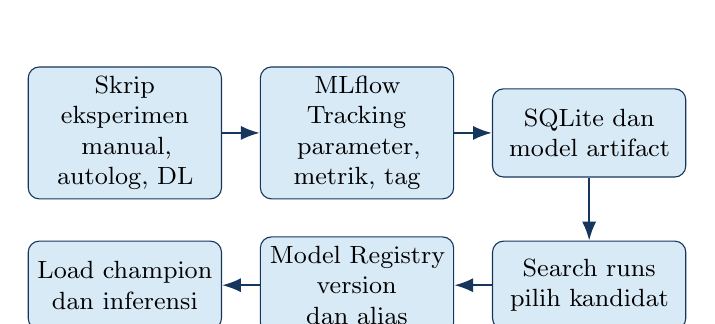
\begin{tikzpicture}[
  node distance=0.48cm,
  box/.style={draw=navy, rounded corners, fill=lightblue, minimum height=1.12cm,
              text width=2.22cm, align=center, font=\small},
  arrow/.style={-{Latex[length=2.4mm]}, thick, draw=navy}
]
  \node[box] (run) {Skrip eksperimen\\manual, autolog, DL};
  \node[box, right=of run] (track) {MLflow Tracking\\parameter, metrik, tag};
  \node[box, right=of track] (store) {SQLite dan\\model artifact};
  \node[box, below=0.8cm of store] (compare) {Search runs\\pilih kandidat};
  \node[box, left=of compare] (registry) {Model Registry\\version dan alias};
  \node[box, left=of registry] (infer) {Load champion\\dan inferensi};
  \draw[arrow] (run) -- (track);
  \draw[arrow] (track) -- (store);
  \draw[arrow] (store) -- (compare);
  \draw[arrow] (compare) -- (registry);
  \draw[arrow] (registry) -- (infer);
\end{tikzpicture}
\end{center}

Kode dipisahkan berdasarkan tugas: \path{basic_tracking.py}, \path{deep_learning.py}, \path{autologging.py}, \path{tune.py}, \path{compare_runs.py}, dan \path{register.py}. Utilitas data, seed, tag, serta konfigurasi MLflow ditempatkan pada \path{common.py} agar seluruh run memakai konteks yang konsisten.

\section{Langkah Praktik dan Hasil}

\subsection{1 --- Menyiapkan Tracking Server}

\texttt{start\_server.sh} mengonfigurasi server dengan SQLite sebagai backend store dan direktori \texttt{mlartifacts/} sebagai artifact store. Pada lingkungan normal, UI tersedia di \url{http://127.0.0.1:5000}. Sandbox praktik menolak pembukaan socket, sehingga eksekusi aktual diarahkan langsung ke SQLite:

\begin{lstlisting}[style=terminal]
export MLFLOW_TRACKING_URI=sqlite:///mlflow.db
\end{lstlisting}

Mode tersebut tetap mendukung pencatatan run, pencarian eksperimen, Model Registry, alias, dan pemuatan model. Perbedaannya adalah UI HTTP tidak aktif selama validasi.

\resultbox{MLflow membuat database lokal dan menyimpan dua run kandidat secara persisten. Tracking serta registry dapat divalidasi tanpa menjalankan layanan HTTP.}

\subsection{2 --- Manual Logging Random Forest}

Skrip \texttt{basic\_tracking.py} melatih Random Forest dengan 200 estimator, kedalaman maksimum 8, dan seed 42. Parameter, tag kandidat, dataset input, hash data, F1, ROC-AUC, \texttt{requirements.txt}, signature, contoh input, serta model dicatat secara eksplisit.

\begin{table}[ht]
\centering
\caption{Hasil validation Random Forest.}
\begin{tabular}{lr}
\toprule
Metrik & Nilai \\
\midrule
Accuracy & 0,956140 \\
Precision & 0,958904 \\
Recall & 0,972222 \\
F1 & 0,965517 \\
ROC-AUC & 0,994048 \\
\bottomrule
\end{tabular}
\hspace{1.3cm}
\begin{tabular}{c|cc}
\multicolumn{3}{c}{\textbf{Confusion matrix}} \\
 & Pred. 0 & Pred. 1 \\
\hline
Aktual 0 & 39 & 3 \\
Aktual 1 & 2 & 70 \\
\end{tabular}
\end{table}

Run tersimpan dengan ID \texttt{c3e105bb4254431faaf17ea5d132905c}. Hasil menunjukkan pemisahan kelas yang baik; hanya lima dari 114 sampel validation salah diklasifikasikan.

\subsection{3 --- Logging Deep Learning per Epoch}

Model PyTorch menggunakan arsitektur MLP 30--64--1, ReLU, dan dropout 0,2. Standardisasi fitur disimpan sebagai buffer di dalam model sehingga model hasil load tetap menerima fitur mentah. Optimizer Adam dimulai pada learning rate 0,0003, kemudian diturunkan 5\% setiap epoch. Metrik \texttt{train\_loss}, \texttt{val\_loss}, \texttt{val\_f1}, \texttt{val\_auc}, dan learning rate disiapkan untuk dicatat pada setiap langkah MLflow.

\begin{center}
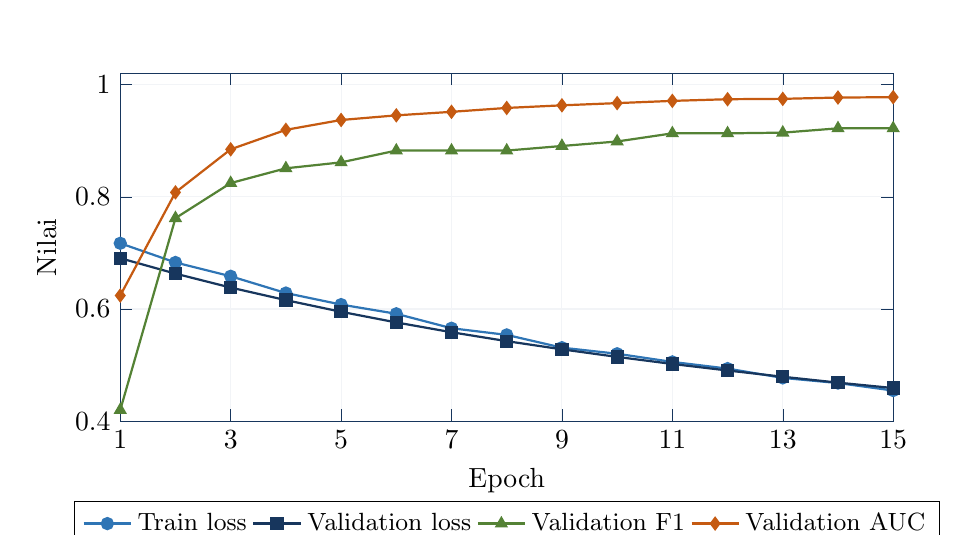
\begin{tikzpicture}
\begin{axis}[
  width=0.94\linewidth,
  height=6.0cm,
  xlabel={Epoch},
  ylabel={Nilai},
  xmin=1,xmax=15,
  ymin=0.4,ymax=1.02,
  xtick={1,3,5,7,9,11,13,15},
  grid=major,
  grid style={draw=lightgray},
  legend style={at={(0.5,-0.23)},anchor=north,legend columns=4,font=\small},
  axis line style={draw=navy},
  tick style={draw=navy}
]
\addplot[thick,blue,mark=*] coordinates {
  (1,.717126) (2,.682933) (3,.658356) (4,.628444) (5,.607903)
  (6,.591485) (7,.565736) (8,.553864) (9,.531088) (10,.520249)
  (11,.505693) (12,.493805) (13,.477205) (14,.468029) (15,.454684)
};
\addlegendentry{Train loss}
\addplot[thick,navy,mark=square*] coordinates {
  (1,.690500) (2,.663056) (3,.638174) (4,.615816) (5,.595054)
  (6,.576073) (7,.558603) (8,.542720) (9,.528115) (10,.514625)
  (11,.502053) (12,.490415) (13,.479259) (14,.468789) (15,.459122)
};
\addlegendentry{Validation loss}
\addplot[thick,green,mark=triangle*] coordinates {
  (1,.420000) (2,.761905) (3,.824427) (4,.850746) (5,.861314)
  (6,.882353) (7,.882353) (8,.882353) (9,.890511) (10,.898551)
  (11,.913043) (12,.913043) (13,.914286) (14,.921986) (15,.921986)
};
\addlegendentry{Validation F1}
\addplot[thick,orange,mark=diamond*] coordinates {
  (1,.624008) (2,.807870) (3,.884590) (4,.919312) (5,.936839)
  (6,.945106) (7,.951389) (8,.958333) (9,.962963) (10,.966931)
  (11,.970899) (12,.973876) (13,.974537) (14,.976852) (15,.977513)
};
\addlegendentry{Validation AUC}
\end{axis}
\end{tikzpicture}
\end{center}

Checkpoint dipilih berdasarkan F1 tertinggi pertama, yaitu epoch ke-14: F1 0,921986, ROC-AUC 0,976852, train loss 0,468029, dan validation loss 0,468789. Pada epoch ke-15 F1 tetap sama dan ROC-AUC naik menjadi 0,977513, tetapi checkpoint tidak diganti karena kriteria utama tidak meningkat.

\resultbox{Pelatihan 15 epoch berhasil dan kurva loss menurun secara konsisten. Integrasi logging MLflow--PyTorch belum dieksekusi dalam satu proses karena environment MLflow tidak memiliki PyTorch, namun fungsi training dan callback pencatatan telah diimplementasikan serta diuji.}

\subsection{4 --- Autologging Scikit-learn}

Skrip \path{autologging.py} menggunakan pipeline \texttt{StandardScaler} dan Logistic Regression. Fungsi \path{mlflow.sklearn.autolog()} menangkap konfigurasi estimator secara otomatis. Hash data, tag tahap, metrik validation domain, signature, dan model dengan nama seragam tetap dicatat manual.

\begin{table}[ht]
\centering
\caption{Hasil validation Logistic Regression.}
\begin{tabular}{lr}
\toprule
Metrik & Nilai \\
\midrule
Accuracy & 0,982456 \\
Precision & 0,986111 \\
Recall & 0,986111 \\
F1 & 0,986111 \\
ROC-AUC & 0,995370 \\
\bottomrule
\end{tabular}
\hspace{1.3cm}
\begin{tabular}{c|cc}
\multicolumn{3}{c}{\textbf{Confusion matrix}} \\
 & Pred. 0 & Pred. 1 \\
\hline
Aktual 0 & 41 & 1 \\
Aktual 1 & 1 & 71 \\
\end{tabular}
\end{table}

Run tersimpan dengan ID \texttt{2bc8487292a9429c89fa3795be02af27}. Model hanya salah pada dua sampel validation dan unggul terhadap Random Forest pada seluruh metrik kecuali tidak ada metrik yang lebih rendah.

\subsection{5 --- Hyperparameter Tuning dengan Optuna}

\texttt{tune.py} mendefinisikan satu parent run dan satu child run untuk setiap trial Optuna. Ruang pencarian Random Forest mencakup \texttt{n\_estimators} 50--300, \texttt{max\_depth} 3--12, dan \texttt{min\_samples\_split} 2--10. Setiap child run mencatat parameter serta validation ROC-AUC; parent run menyimpan parameter dan model terbaik.

\begin{lstlisting}[style=terminal]
python -m src.tune --trials 20
# parent run -> trial-000 ... trial-019
\end{lstlisting}

Tahap ini telah diimplementasikan, tetapi tidak dieksekusi karena Optuna tidak tersedia pada environment lokal dan pemasangan dari PyPI terhalang akses jaringan. Oleh karena itu, laporan tidak mencantumkan parameter atau skor tuning fiktif.

\subsection{6 --- Membandingkan dan Memilih Run}

\texttt{compare\_runs.py} menggunakan MLflow search API untuk mengambil run bertag \texttt{candidate=true} dan memiliki \texttt{val\_auc}. Kandidat diurutkan berdasarkan ROC-AUC, kemudian F1 sebagai pemecah seri. Hasil pilihan ditulis ke \texttt{selected\_run.json} agar tahap registry tidak bergantung pada pemilihan manual.

\begin{center}
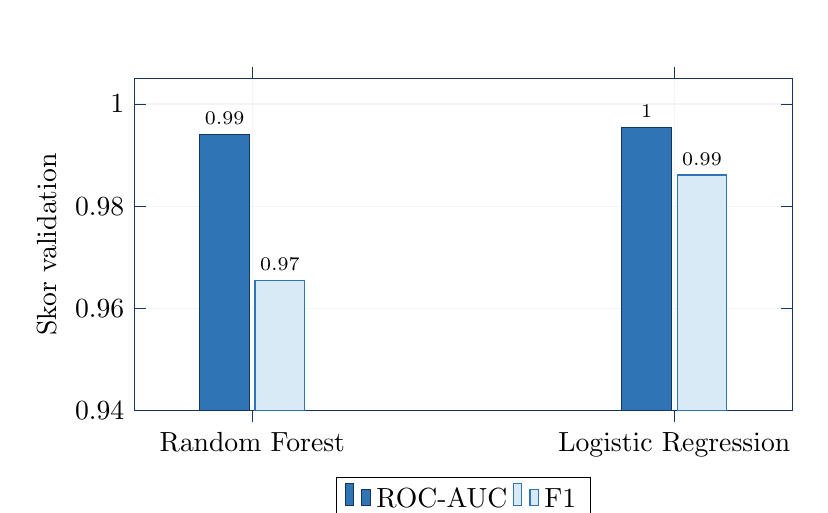
\begin{tikzpicture}
\begin{axis}[
  ybar,
  bar width=18pt,
  width=0.82\linewidth,
  height=5.8cm,
  ymin=0.94,ymax=1.005,
  ylabel={Skor validation},
  symbolic x coords={Random Forest,Logistic Regression},
  xtick=data,
  enlarge x limits=0.28,
  legend style={at={(0.5,-0.2)},anchor=north,legend columns=2},
  nodes near coords,
  nodes near coords style={font=\scriptsize},
  grid=major,
  grid style={draw=lightgray},
  axis line style={draw=navy},
  tick style={draw=navy}
]
\addplot[fill=blue,draw=navy] coordinates {(Random Forest,.994048) (Logistic Regression,.995370)};
\addlegendentry{ROC-AUC}
\addplot[fill=lightblue,draw=blue] coordinates {(Random Forest,.965517) (Logistic Regression,.986111)};
\addlegendentry{F1}
\end{axis}
\end{tikzpicture}
\end{center}

\resultbox{Logistic Regression terpilih dengan ROC-AUC 0,995370 dan F1 0,986111. Selisih AUC terhadap Random Forest hanya 0,001323, tetapi selisih F1 mencapai 0,020594.}

\subsection{7 --- Model Registry, Alias, dan Inferensi}

\path{register.py} membaca run pilihan dan mendaftarkan model dengan nama berikut:

\begin{lstlisting}[style=terminal]
handson-1-breast-cancer-clf
\end{lstlisting}

Skrip lalu menetapkan alias \texttt{challenger} dan \texttt{champion}. Aplikasi memuat model menggunakan URI stabil:

\begin{lstlisting}[style=terminal]
models:/handson-1-breast-cancer-clf@champion
\end{lstlisting}

Eksekusi menghasilkan model version 1; kedua alias menunjuk ke versi tersebut dan sumber model tetap terhubung ke run Logistic Regression. Model champion berhasil dimuat kembali dan menghasilkan contoh prediksi \texttt{[0, 1, 0]} untuk tiga baris input.

\resultbox{Siklus dari eksperimen ke registry berhasil. Alias membuat kode inferensi tidak perlu mengetahui nomor versi; pergantian champion dapat dilakukan pada registry tanpa mengubah URI aplikasi.}

\section{Validasi dan Keterbatasan}

\begin{table}[ht]
\centering
\small
\caption{Status validasi implementasi Hands-on 1.}
\begin{tabularx}{\linewidth}{>{\bfseries\raggedright\arraybackslash}p{0.31\linewidth}>{\raggedright\arraybackslash}p{0.16\linewidth}>{\raggedright\arraybackslash}X}
\toprule
Komponen & Status & Bukti atau keterangan \\
\midrule
Manual tracking Random Forest & \statusok & Run, metrik, model, signature, dan artifact tersimpan \\
Autologging Logistic Regression & \statusok & Run dan model tersimpan; menjadi kandidat terbaik \\
Search dan seleksi run & \statusok & Logistic Regression dipilih secara programatik \\
Model Registry dan alias & \statusok & Version 1; alias challenger dan champion \\
Load model dan inferensi & \statusok & URI champion dimuat; prediksi \texttt{[0, 1, 0]} \\
Training PyTorch & \statuspartial & 15 epoch selesai; logging MLflow lintas environment belum dijalankan \\
Optuna nested runs & \statuspending & Kode tersedia; paket Optuna tidak tersedia \\
Tracking server HTTP/UI & \statuspending & Sandbox menolak pembukaan socket; direct SQLite berhasil \\
Unit test dan compile check & \statusok & Tiga test lulus; seluruh modul dapat dikompilasi \\
\bottomrule
\end{tabularx}
\end{table}

Keterbatasan utama berasal dari environment, bukan dari rancangan kode. MLflow dan PyTorch tersedia pada environment Python yang berbeda, Optuna tidak terpasang, serta sandbox tidak mengizinkan proses membuka port. Percobaan pemasangan paket juga gagal karena resolusi jaringan. Karena itu, status pada tabel membedakan hasil yang benar-benar tersimpan di MLflow dari fungsi yang baru divalidasi secara lokal.

\section{Pembahasan}

Manual logging memberi kendali penuh atas nama parameter, metrik, tag, dan artifact, tetapi membutuhkan kode lebih banyak. Autologging mengurangi boilerplate dan tetap dapat digabung dengan pencatatan manual untuk informasi domain seperti hash data dan label kandidat. Pada eksperimen ini, pipeline Logistic Regression yang lebih sederhana justru memberikan F1 dan ROC-AUC terbaik.

Logging per epoch diperlukan untuk membaca dinamika deep learning yang tidak terlihat dari satu metrik akhir. Kurva menunjukkan loss training dan validation menurun bersama tanpa tanda divergensi yang jelas selama 15 epoch. F1 meningkat tajam pada awal training lalu melandai, sehingga penambahan epoch perlu dievaluasi berdasarkan manfaat dan biaya komputasi.

Nested runs pada Optuna memisahkan ringkasan studi dari detail setiap trial. Struktur tersebut memudahkan perbandingan parameter tanpa memenuhi daftar eksperimen utama dengan run yang tidak memiliki hubungan. Selanjutnya, pemilihan programatik dan alias registry membentuk batas yang jelas antara eksperimen dan konsumsi model oleh aplikasi.

\section{Kesimpulan}

Hands-on 1 berhasil menerapkan fondasi experiment tracking dan pengelolaan model menggunakan MLflow. Dua run kandidat tercatat pada SQLite. Logistic Regression terpilih sebagai model terbaik dengan ROC-AUC 0,995370 dan F1 0,986111. Model diregistrasikan sebagai \path{handson-1-breast-cancer-clf} versi 1, diberi alias \texttt{champion}, serta berhasil dimuat kembali untuk inferensi.

Praktik menunjukkan bahwa reproducibility tidak hanya bergantung pada algoritma. Seed, hash data, parameter, metrik, signature, artifact, dan hubungan run ke model version perlu dicatat bersama. MLflow autologging mempercepat pencatatan standar, sedangkan manual logging tetap penting untuk konteks domain. Logging PyTorch dan tuning Optuna sudah disiapkan dalam desain yang sama, tetapi validasi penuh keduanya membutuhkan environment terpadu yang menyediakan MLflow, PyTorch, dan Optuna serta mengizinkan tracking server berjalan.

\appendix
\section{Perintah Reproduksi}

\begin{lstlisting}[style=terminal]
cd handson-1
python -m venv --system-site-packages .venv
source .venv/bin/activate
pip install -r requirements.txt

# Terminal 1: jalankan server dan UI
./start_server.sh

# Terminal 2: jalankan seluruh tahap
export MLFLOW_TRACKING_URI=http://127.0.0.1:5000
./run_pipeline.sh
\end{lstlisting}

Jika layanan HTTP tidak dapat dibuka, backend SQLite dapat dipakai langsung:

\begin{lstlisting}[style=terminal]
export MLFLOW_TRACKING_URI=sqlite:///mlflow.db
python -m src.basic_tracking
python -m src.autologging
python -m src.deep_learning --epochs 15
python -m src.tune --trials 20
python -m src.compare_runs
python -m src.register
\end{lstlisting}

Validasi kode dijalankan dengan:

\begin{lstlisting}[style=terminal]
python -m unittest discover -s tests -v
python -m compileall -q src tests
\end{lstlisting}

\end{document}
